% Autheur: Amaury JOlY

\subsubsection{Definition}
Les réserves de liquidité sont des marchés automatisés qui permettent aux utilisateurs de fournir des liquidités pour les échangeurs décentralisés (\acrshort{dex}) et de 
remporter une comission à chaque transaction \cite{jensen2021introduction, belchior2022survey, augustin2022yield}. 
Les fournisseurs de liquidités déposent des fonds dans une réserve de liquidité et reçoivent des jetons 
LP\footnote{Liquidity Provider Token} en retour. Les jetons LP représentent une part de propriété dans la réserve de liquidité et peuvent être utilisés pour 
retirer des fonds de la réserve. Les réserves de liquidité sont un concept clé de l’écosystème DeFi. Il permettent la mise en place d'échangeurs décentralisés 
qui donne la possibilité aux utilisateurs d’échanger des actifs sans avoir besoin d’un intermédiaire centralisé. \\
A chaque échange réalisé via la réserve, les possesseurs de liquidités recoivents des récompenses qui sont les frais d'échanges des utilisateurs. Les récompenses 
sont généralement des jetons de gouvernance ou des jetons de protocole. Les réserves de liquidité se régulent ainsi en ajustant les frais de transaction 
en fonction de l’offre et de la demande. Si la demande pour une réserve de liquidité particulier est élevée, les frais de transaction augmentent pour encourager 
les fournisseurs de liquidités à déposer plus de fonds dans la réserve. Si la demande est faible, les frais de transaction diminuent pour encourager les 
utilisateurs à échanger des actifs sur la réserve de liquidité. \\
Une réserve de liquidité repose sur un smart contract et bénéficie ainsi de la décentralisation et de la sécurité de la \gls{blockchain} sur laquelle il repose.
\begin{figure}[h!]
    \centering
    \stackunder{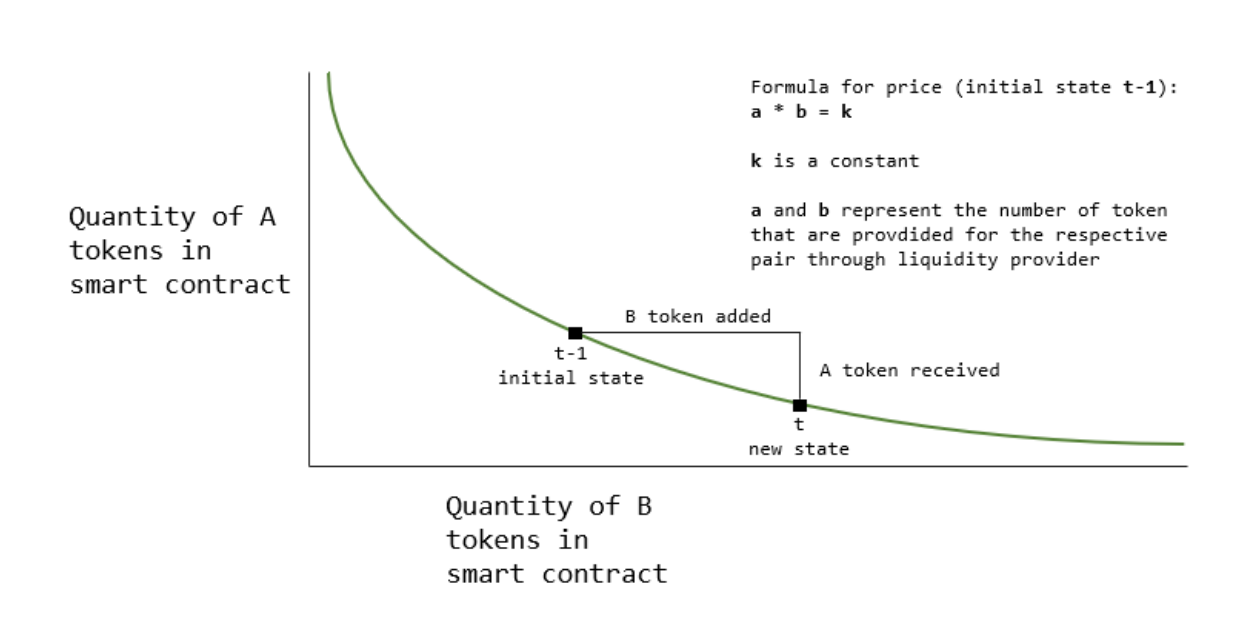
\includegraphics[scale=0.3]{decentralisation/reserve_liquidite.png}}
    {\scriptsize Source: An introduction to decentralized finance (defi) \cite{jensen2021introduction} }
    \caption{Marché de la reserve de liquidité}
    \label{fig:liquidite}
\end{figure}

\subsubsection{Exemple: PancakeSwap}
PancakeSwap est une plateforme d’échange décentralisée (DEX) qui repose sur la \gls{blockchain} Binance Smart Chain. \cite{augustin2022yield} Elle permet aux utilisateurs d’échanger des 
cryptomonnaies de manière décentralisée. Le jeton natif de la plateforme PancakeSwap, le CAKE, est utilisé 
pour la gouvernance du protocole. Ainsi, grâce à lui, vous pouvez voter pour des propositions soumises par la communauté. La sécurité de PancakeSwap est assurée 
par un ensemble de smart contracts permettant de sécuriser les transactions et les échanges de manière décentralisée. Les réserves de liquidités sont un 
élément clé de PancakeSwap. Ils permettent aux utilisateurs de fournir des liquidités à la plateforme et de recevoir des récompenses en échange. Les réserves 
de liquidités sont également utilisés pour déterminer le prix des actifs sur la plateforme.

\subsubsection{Limitations}
Les réserves de liquidités présentent certaines limites \cite{caldarelli2021blockchain}. Tout d’abord, les réserves de liquidités sont vulnérables aux attaques de liquidités. Les attaques 
de liquidités sont des attaques dans lesquelles un utilisateur manipule le prix d’un actif en ajoutant ou en retirant une grande quantité de liquidités d’une 
réserve. Cela peut entraîner une baisse significative du prix de l’actif et des pertes pour les fournisseurs de liquidités. De plus, les réserves de liquidités 
peuvent être affectés par des problèmes de liquidité. Si une réserve de liquidités n’a pas suffisamment de liquidités, il peut être difficile pour les 
utilisateurs d’acheter ou de vendre des actifs sur la plateforme. Enfin, les réserves de liquidités peuvent être affectés par des problèmes de sécurité. Si 
une réserve de liquidités est compromise, les utilisateurs peuvent perdre leurs fonds. \\
Un exemple d'attaque sur une réserve de liquidité est la CVE-2021-3006 \cite{nvd2021-3006,blocksec2021Seal}. La CVE-2021-3006 est une vulnérabilité de sécurité qui a été exploitée en décembre 
2020 et janvier 2021. Elle concerne un manquement de controle d'accès dans l’implémentation du \textit{\gls{smart contract}} pour une réserve de liquidité en lien avec 
Seal Finance (Seal), un jeton \gls{Ethereum}. Cette vulnérabilité permet une manipulation des prix ayant permis à l'attaquant de réaliser une plus-value artificiel 
sur ses jetons.
